\pdfoutput=1
\documentclass[10pt,twocolumn]{article}
\usepackage[letterpaper,margin=0.75in,columnsep=0.25in]{geometry}
\usepackage[T1]{fontenc}
\usepackage{mathptmx}
\usepackage{amsmath,amssymb}
\usepackage{booktabs}
\usepackage{array}
\usepackage{graphicx}
\usepackage{xcolor}
\usepackage[numbers,sort&compress]{natbib}
\usepackage{url}\def\UrlBreaks{\do\/}\def\UrlBigBreaks{}\def\UrlNoBreaks{\do\:\do\(\do\[\do\{\do\<}
\hyphenation{Paged-Attention Radix-Attention Cached-Attention LMCache Mooncake EfficientAgent CONCUR TokenCake HotCarbon}
\makeatletter\setlength{\@fptop}{0pt}\makeatother
\usepackage[hidelinks]{hyperref}
\hypersetup{pdftitle={The Agent Memory Wall: Measuring and Managing the GPU Energy of KV Caches for AI Agents},
  pdfauthor={Bharat Bhushan Sharma}}
\usepackage{microtype}
\usepackage{caption}
\usepackage{tikz}
\usetikzlibrary{arrows.meta,positioning,shapes.geometric}
\captionsetup{font=small,labelfont=bf}
\setlength{\tabcolsep}{4pt}
\raggedbottom

\newcommand{\Cgpu}{C}
\newcommand{\WC}{W/C}

\title{\Large\bfseries The Agent Memory Wall:\\ Measuring and Managing the GPU Energy of KV Caches for AI Agents}
\author{Bharat Bhushan Sharma\\ \small PHENEX TECHNOLOGIES INC (WattOps), Vancouver, Canada\\ \small bharat@wattops.dev}
\date{}

\begin{document}
\maketitle

\begin{abstract}
An AI agent alternates between model calls and tool calls. While a tool runs, the serving engine keeps the agent's
key--value (KV) cache only if nothing else needs the memory; when it is evicted, the next call recomputes the whole
context. We measure what this costs in GPU energy on an H200 with vLLM and SGLang, three Qwen3 models (32B, 30B-A3B
and 8B) and four workloads: synthetic sessions, recorded SWE-agent trajectories, replayed samples of production
tool-agent traffic from Kimi, and graded BFCL multi-turn tasks. Every prediction was registered before its run.

We report four results. First, on synthetic sessions, once the agents' working set exceeds the cache by a factor of 1.2--2.2, hits collapse;
past that point energy per turn is within 0.01--1.6\% of running without a cache. With
Qwen3-32B and 5\,s pauses the collapse comes between 16 and 32 sessions of about 11k tokens and between 8 and 16 of
about 27k. Second, restoring a prompt's KV from host memory takes about 1/110 to 1/220 of the above-idle GPU energy of
recomputing it. Third, on a 1/4 sample of the production trace, which overloads the GPU, a 160\,GB host tier let the GPU
finish every request (85--86\% with the GPU cache) and process 16--18\% more prompt tokens for about the same energy, in two
time windows; on a lighter 1/8 sample the tier saved under 1\%. Given measured hit rates, a one-parameter model predicts the busy card's energy per
token to within about 1\%. Fourth, on synthetic sessions, an admission gate, switched on only when the working set
exceeds 1.2 times the cache, cost no energy below that point; above it, in two 10-minute runs, it served every session,
completed 48--62\% more turns and cut energy per turn by 42--50\%, at the price of minutes of queueing at
admission. On BFCL, accuracy with and without the cache differed by 3 of 400 tasks, and the
cache doubled correct answers per kWh. All energy is GPU board energy.
\end{abstract}

\section{Introduction}

An AI agent sends its whole history to a language model, waits for an answer, runs a tool, appends the result and
calls the model again. Each call repeats a long prefix the server has already processed. Serving engines keep the
attention keys and values of that prefix (the KV cache) so that the next call does not recompute them, and the saving
is large: for a 32-billion-parameter model we measure 56--73\,mJ of above-idle GPU energy per recomputed prompt token and
almost nothing per cached one.

The cache has a weakness that agents expose. The engine does not know that an agent has gone to run a tool or how long
it will be away, so it keeps KV by recency and evicts the least recently used entry when memory runs out. Once the agents'
working set exceeds the cache by a factor between 1.2 and 2.2, depending on how long they pause, hits collapse until nearly every agent's KV is evicted before it returns. Prior work has named this collapse
(``middle-phase thrashing'' in CONCUR~\cite{chen2026concur}), located it~\cite{he2026robot,lu2026metastability} and
shown that a host-memory tier helps only when it holds the agents' working set~\cite{shao2026efficientagent}. All of
that work reports latency or throughput. Energy has been measured for KV offloading (at low concurrency, across
buffer sizes of 8--128\,GiB, on production agent traces)~\cite{mao2026offloading} and for prefix reuse on single
requests~\cite{shewale2026prefixbench}, but not through the collapse that many concurrent agents cause, and not for
the admission rules proposed to prevent it.

We report measurements, a small model that predicts them, and an admission gate built from the model. We ran
everything on one NVIDIA H200 NVL with two unmodified engines (vLLM and SGLang) and three models of different shapes (a
dense 32B model, a 30B mixture-of-experts (MoE) model and a dense 8B model); only the 10-minute adaptive-gate runs used a second H200 NVL host. The workloads go from controlled to real:
synthetic sessions whose size and pauses we set, 400 recorded SWE-agent trajectories, a replay of 1/8 and 1/4 samples of two 15-minute windows of
Kimi's one-hour production tool-agent trace, with their original timing and prefix sharing, and 400 graded tasks from the
Berkeley Function Calling Leaderboard (BFCL) multi-turn benchmark. We wrote each prediction down before the run that
tested it (Appendix~\ref{app:prereg}) and kept the ones that failed.

Figure~\ref{fig:arch} shows the paths a prompt token can take and where the gate sits.

\begin{figure*}[t]
\centering
\frenchspacing
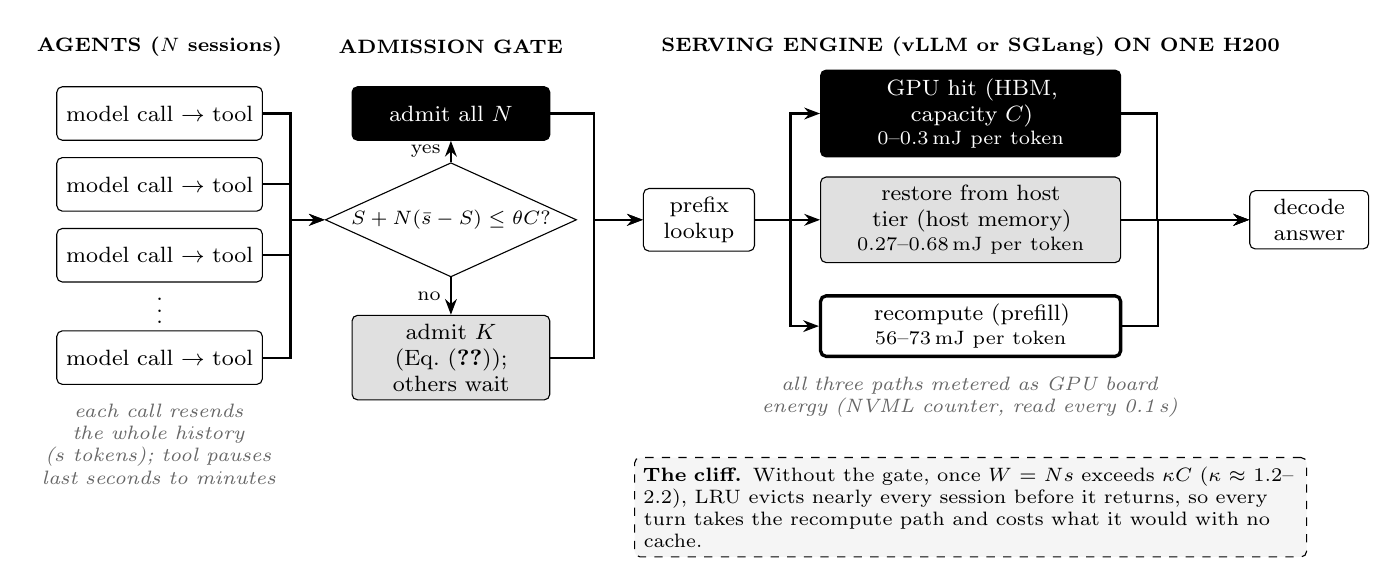
\begin{tikzpicture}[
  font=\footnotesize,
  box/.style={draw, rounded corners=2pt, align=center, inner sep=3pt, minimum height=0.68cm,
    execute at begin node={\hyphenpenalty=10000\exhyphenpenalty=10000}},
  dark/.style={box, fill=black, text=white},
  grey/.style={box, fill=black!12},
  light/.style={box, fill=white},
  arr/.style={-{Stealth[length=2mm]}, thick},
  lab/.style={font=\scriptsize\itshape, text=black!60, align=center,
    execute at begin node={\hyphenpenalty=10000\exhyphenpenalty=10000}},
  head/.style={font=\scriptsize\bfseries, align=left}
]
% ---------- agents
\node[head] at (1.3,2.65) {AGENTS ($N$ sessions)};
\node[light, text width=2.4cm] (a1) at (1.3,1.8) {model call $\rightarrow$ tool};
\node[light, text width=2.4cm] (a2) at (1.3,0.9) {model call $\rightarrow$ tool};
\node[light, text width=2.4cm] (a3) at (1.3,0.0) {model call $\rightarrow$ tool};
\node at (1.3,-0.6) {$\vdots$};
\node[light, text width=2.4cm] (an) at (1.3,-1.3) {model call $\rightarrow$ tool};
\node[lab, anchor=north, text width=3.0cm] at ([yshift=-0.12cm]an.south) {each call resends the whole history ($s$~tokens); tool pauses last seconds to minutes};

% ---------- gate
\node[head] at (5.0,2.65) {ADMISSION GATE};
\node[dark, text width=2.3cm] (all) at (5.0,1.8) {admit all $N$};
\node[diamond, draw, aspect=2.2, inner sep=0.5pt, align=center, fill=white, font=\scriptsize] (dec) at (5.0,0.45)
  {$S+N(\bar s-S)\le\theta C$?};
\node[grey, text width=2.3cm] (k) at (5.0,-1.3) {admit $K$ (Eq.~\eqref{eq:gate});\\others wait};
\draw[arr] (dec.north) -- node[left, font=\scriptsize]{yes} (all.south);
\draw[arr] (dec.south) -- node[left, font=\scriptsize]{no} (k.north);
\draw[arr] (a1.east) -- ++(0.35,0) |- (dec.west);
\draw[arr] (an.east) -- ++(0.35,0) |- (dec.west);
\draw[thick] (a2.east) -- ++(0.35,0);
\draw[thick] (a3.east) -- ++(0.35,0);

% ---------- engine
\node[head] at (11.6,2.65) {SERVING ENGINE (vLLM or SGLang) ON ONE H200};
\node[light, text width=1.2cm] (lk) at (8.15,0.45) {prefix\\lookup};
\draw[arr] (all.east) -- ++(0.55,0) |- (lk.west);
\draw[arr] (k.east) -- ++(0.55,0) |- (lk.west);

\node[dark, text width=3.6cm] (hit) at (11.6,1.8) {GPU hit (HBM, capacity $C$)\\[-1pt]{\scriptsize 0--0.3\,mJ per token}};
\node[grey, text width=3.6cm] (res) at (11.6,0.45) {restore from host tier (host memory)\\[-1pt]{\scriptsize 0.27--0.68\,mJ per token}};
\node[light, text width=3.6cm, very thick] (rec) at (11.6,-0.9) {recompute (prefill)\\[-1pt]{\scriptsize 56--73\,mJ per token}};
\draw[arr] (lk.east) -- ++(0.45,0) |- (hit.west);
\draw[arr] (lk.east) -- (res.west);
\draw[arr] (lk.east) -- ++(0.45,0) |- (rec.west);

\node[light, text width=1.3cm] (out) at (15.9,0.45) {decode\\answer};
\draw[arr] (hit.east) -- ++(0.45,0) |- (out.west);
\draw[arr] (res.east) -- (out.west);
\draw[arr] (rec.east) -- ++(0.45,0) |- (out.west);

\node[lab, anchor=north, text width=5.4cm] (meter) at ([yshift=-0.12cm]rec.south) {all three paths metered as GPU board energy (NVML counter, read every 0.1\,s)};

% ---------- cliff callout
\node[draw, dashed, rounded corners=2pt, align=left, font=\scriptsize, text width=8.3cm, fill=black!4] at (11.6,-3.2)
{\textbf{The cliff.} Without the gate, once $W=Ns$ exceeds $\kappa C$ ($\kappa\approx1.2$--2.2), LRU evicts nearly every
session before it returns, so every turn takes the recompute path and costs what it would with no cache.};
\end{tikzpicture}
\caption{What happens to one agent turn. Agents resend their history after each tool call. The admission gate
(Section~\ref{sec:control}) admits every session while the working set fits under $\theta C$ and only $K$ sessions
otherwise ($S$, $\bar s$, $\theta$, $\kappa$ and $K$ are defined in Section~\ref{sec:model}). In the engine, each prompt token takes one of three paths whose above-idle GPU energy we measured
(Section~\ref{sec:cost}): its KV is still in GPU memory, in a host tier, or gone. HBM: the GPU's high-bandwidth memory; LRU: least-recently-used eviction; NVML: NVIDIA Management Library.}
\label{fig:arch}
\end{figure*}


\paragraph{Findings.}
\begin{enumerate}
\item \textbf{Past the cliff, a full cache saves almost no energy.} GPU energy per turn equals that of running with no cache,
to within 0.01--1.6\% in every cell past the cliff we measured (vLLM: three models and two context lengths; SGLang: Qwen3-32B). The cliff falls where the agents'
working set $W$ exceeds the cache capacity $C$ by a factor of 1.2--2.2: hits fall to half their 16-session level at 1.2 and vanish by 1.55 with 5\,s pauses, and fall to
half at 1.5 and vanish by 2.2 with 30\,s pauses. With sessions 2.5 times longer (27k instead of 11k tokens) the cliff moved from between 16 and 32 sessions to between 8 and 16, consistent with the $1/s$ scaling of Eq.~\eqref{eq:cliff} (Section~\ref{sec:cliff}).
\item \textbf{Holding KV costs no measurable power; rebuilding it does.} A full cache changed idle power by less than
0.2\%, and restoring a prompt's KV from host memory took 1/110 to 1/220 of the above-idle GPU energy of recomputing it,
with the gap growing with context length (Section~\ref{sec:cost}).
\item \textbf{On production traffic, a host tier adds capacity.} In a replay of Kimi's tool-agent trace, a 160\,GB host
tier let one H200 finish every request where the GPU cache alone finished 85--86\%, and process 16--18\% more prompt tokens
for about the same GPU energy (15--17\% less per prompt token), in two time windows of a 1/4 sample that overloads the
card; on a 1/8 sample, which the GPU cache served in full, the tier saved under 1\% (Sections~\ref{sec:tiers}
and~\ref{sec:production}).
\item \textbf{The energy is predictable on a busy GPU.} A one-parameter model fitted on synthetic sessions predicts the
production energy ratios to within about 1\% when the GPU is saturated, and a block-level hit-rate predictor run on
hashed request logs matches the measured hit rate to within 0.04--4.3 percentage points when the GPU keeps up. The model fails at
light load and the predictor under overload; we report both (Sections~\ref{sec:model} and~\ref{sec:production}).
\item \textbf{A gate that acts only under pressure costs nothing below the cliff and saves energy above it.} Admitting every agent while the working set is at most 1.2 times the cache, and
$K$ agents from Eq.~\eqref{eq:gate} above that, cost no energy below the cliff, with 90th-percentile resume latency no worse. Above it, in 150\,s
steps, it cut energy per turn by 41--45\% but left a third to a half of the sessions unserved at the highest loads; in
600\,s steps it served every session, completed 48--62\% more turns and cut energy per turn by 42--50\%, at the price of
queueing: the 90th percentile of first-turn latency was 1.9--2.7 times the GPU cache's (Section~\ref{sec:control}).
\item \textbf{On graded tasks, the cache doubled correct answers per kWh.} On BFCL, accuracy with and without the cache differed by 3 of 400 tasks (204 correct with the cache,
201 without; one round) and halved time and energy: 2.0$\times$ the correct answers per kWh (Section~\ref{sec:accuracy}).
\end{enumerate}

\paragraph{What is not new.} Thrashing, the cliff, the weakness of eviction policies, host-tier sizing by working set
and working-set admission control are all published~\cite{chen2026concur,he2026robot,lu2026metastability,
shao2026efficientagent,denning1968working}, and so are offloading during tool calls~\cite{xia2026mori,tokencake2025}
and hit-rate prediction from traces~\cite{kvset2026}. Our contribution is to measure these in GPU energy, on one
hardware platform and one set of workloads, including production traffic; to show how far a simple model predicts them; and to report where
the published ideas fail in practice (Section~\ref{sec:control}). All energy figures are GPU board energy read from
the energy counter of NVML (the NVIDIA Management Library). We could not meter host CPU and memory energy in our rented container, and we do not convert
our percentages to whole-server savings (Section~\ref{sec:discussion}, Limitations).

\begin{figure*}[t]
\centering
\frenchspacing
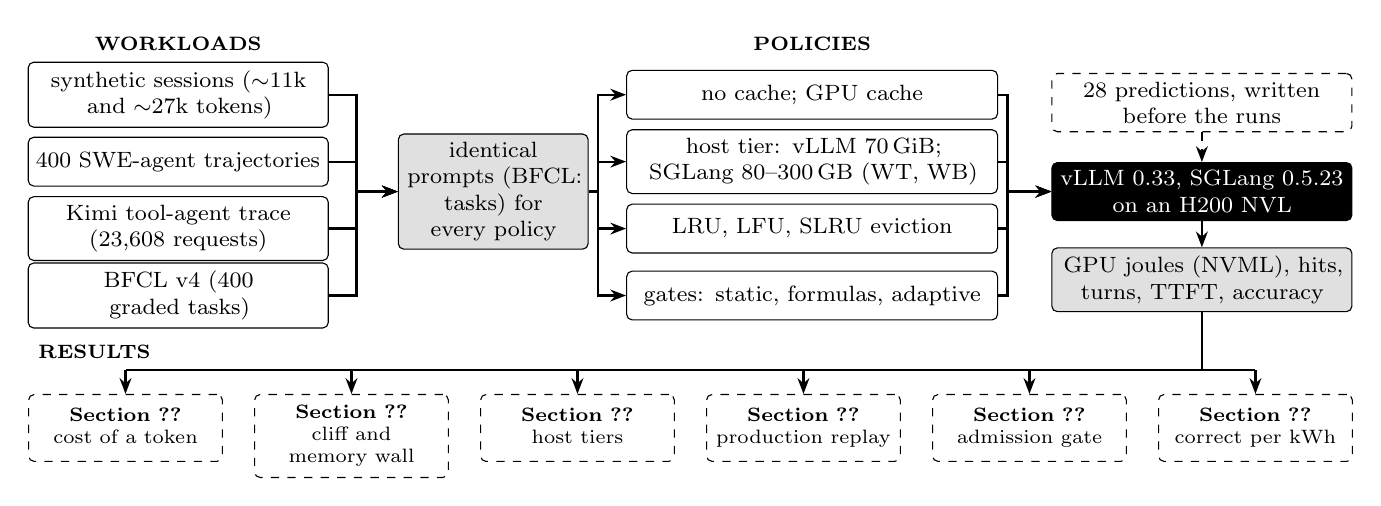
\begin{tikzpicture}[
  font=\footnotesize,
  box/.style={draw, rounded corners=2pt, align=center, inner sep=3pt, minimum height=0.62cm,
    execute at begin node={\hyphenpenalty=10000\exhyphenpenalty=10000}},
  dark/.style={box, fill=black, text=white},
  grey/.style={box, fill=black!12},
  light/.style={box, fill=white},
  arr/.style={-{Stealth[length=2mm]}, thick},
  head/.style={font=\scriptsize\bfseries, align=left}
]
% ---------- workloads
\node[head] at (1.75,3.3) {WORKLOADS};
\node[light, text width=3.6cm] (w1) at (1.75,2.65) {synthetic sessions ($\sim$11k and $\sim$27k tokens)};
\node[light, text width=3.6cm] (w2) at (1.75,1.8) {400 SWE-agent trajectories};
\node[light, text width=3.6cm] (w3) at (1.75,0.95) {Kimi tool-agent trace (23,608 requests)};
\node[light, text width=3.6cm] (w4) at (1.75,0.1) {BFCL v4 (400 graded tasks)};
\node[grey, text width=2.2cm] (same) at (5.75,1.42) {identical prompts (BFCL: tasks) for every policy};
\foreach \i in {1,2,3,4} \draw[arr] (w\i.east) -- ++(0.35,0) |- (same.west);

% ---------- policies
\node[head] at (9.8,3.3) {POLICIES};
\node[light, text width=4.5cm] (p1) at (9.8,2.65) {no cache; GPU cache};
\node[light, text width=4.5cm] (p2) at (9.8,1.8) {host tier: vLLM 70\,GiB; SGLang 80--300\,GB (WT, WB)};
\node[light, text width=4.5cm] (p3) at (9.8,0.95) {LRU, LFU, SLRU eviction};
\node[light, text width=4.5cm] (p4) at (9.8,0.1) {gates: static, formulas, adaptive};
\foreach \i in {1,2,3,4} \draw[arr] (same.east) -- ++(0.12,0) |- (p\i.west);

% ---------- engine, predictions, measurement
\node[box, dashed, text width=3.6cm] (pre) at (14.75,2.55) {28 predictions, written before the runs};
\node[dark, text width=3.6cm] (eng) at (14.75,1.42) {vLLM 0.33, SGLang 0.5.23\\on an H200 NVL};
\node[grey, text width=3.6cm] (meas) at (14.75,0.3) {GPU joules (NVML), hits, turns, TTFT, accuracy};
\foreach \i in {1,2,3,4} \draw[arr] (p\i.east) -- ++(0.12,0) |- (eng.west);
\draw[arr, dashed] (pre) -- (eng);
\draw[arr] (eng) -- (meas);

% ---------- results
\node[head, anchor=west] at (-0.15,-0.62) {RESULTS};
\draw[thick] (meas.south) -- (14.75,-0.85);
\draw[thick] (1.08,-0.85) -- (15.43,-0.85);
\foreach \x/\s/\t [count=\j] in {1.08/{\ref{sec:cost}}/{cost of a token},
                      3.95/{\ref{sec:cliff}}/{cliff and memory wall},
                      6.82/{\ref{sec:tiers}}/{host tiers},
                      9.69/{\ref{sec:production}}/{production replay},
                      12.56/{\ref{sec:control}}/{admission gate},
                      15.43/{\ref{sec:accuracy}}/{correct per kWh}} {
  \node[box, dashed, text width=2.25cm, minimum height=0.85cm, anchor=north, font=\scriptsize] (r\j) at (\x,-1.15) {\textbf{Section~\s}\strut\\\t\strut};
  \draw[arr] (\x,-0.85) -- (r\j.north);
}
\end{tikzpicture}
\caption{Method. Four workloads, from controlled to real, are sent with identical prompts (for BFCL, identical tasks) to every policy on two
engines and one GPU type\@. Every run records GPU energy from the NVML counter, cache hits, completed turns or requests,
latency and, for BFCL, graded accuracy. Each prediction was written before its run (Appendix~\ref{app:prereg}). WT/WB: write-through/write-back host tier; LFU/SLRU: least-frequently-used/segmented-LRU eviction; TTFT: time to first token.}
\label{fig:workflow}
\end{figure*}


\section{Setup and method}
\label{sec:setup}

\paragraph{Terms.} A \emph{policy} is one cache configuration under test. A session's size $s$ is the number of tokens of
KV it holds; the \emph{working set} $W$ is the KV the open sessions need at once, and the \emph{cliff} is the load at
which the cache's hit rate collapses. \emph{GPU cache} (``GPU'' in some tables) is the engine's default prefix cache in GPU memory with no
host tier; \emph{no cache} turns prefix caching off; a \emph{host tier} keeps evicted or copied KV in host memory. LRU,
LFU and SLRU are least-recently-used, least-frequently-used and segmented-LRU eviction. TTFT is the time to the first
output token; \emph{resume latency} is the TTFT of a session's later turns plus any wait for admission; p90 is the 90th
percentile. A \emph{step} is one measured period at a fixed configuration; in the production replay
the \emph{drain} is the 240\,s after a window ends during which running requests may finish. AIMD is
additive-increase, multiplicative-decrease window control. Figure~\ref{fig:workflow} summarizes the method.

\paragraph{Hardware and engines.} Except where noted, all runs used one NVIDIA H200 NVL (141\,GB of high-bandwidth memory, HBM; PCIe Gen5 $\times$16 to the host) rented
as a container that could use up to 454\,GiB of host memory. The 10-minute adaptive-gate runs (Section~\ref{sec:control}) used a second H200 NVL host with the same
engine and meter versions (driver 595, idle 97\,W). We ran vLLM 0.33 and SGLang 0.5.23 without modification, with prefix
caching on (vLLM's automatic prefix caching; SGLang's radix cache) unless a run turned it off. vLLM used 90\% of GPU
memory and SGLang 88\%. Host-memory tiers were vLLM's KV offloading and SGLang's hierarchical cache (HiCache) in its
default write-through (WT) mode, and in write-back (WB) mode where stated.

\paragraph{Models.} Qwen3-32B (dense, 64 layers, 64 query and 8 KV heads of dimension 128; 256\,KiB of KV per token in BF16),
Qwen3-30B-A3B (mixture of experts, 48 layers, 4 KV heads; 96\,KiB per token) and Qwen3-8B (dense; 144\,KiB per
token)~\cite{qwen3}, all in BF16\@. After weights, the engines' GPU KV capacity $C$ was 244,928 tokens for Qwen3-32B on
vLLM (251,423 on SGLang), 704,032 for Qwen3-30B-A3B on vLLM, and 777,872 for Qwen3-8B on vLLM (780,230 on SGLang), as
reported in each engine's startup log.

\paragraph{Energy.} We read the GPU's cumulative energy counter through NVML every 0.1\,s with \texttt{joules}, our open-source
meter, and attributed to each step the energy between its start and end. Before each engine's measured steps we sent
four warm-up requests, waited until GPU temperature varied by less than 1\,\textdegree C over 60\,s, and measured 30\,s of
idle power. Every energy figure in this paper is GPU board energy. The container hid the CPU's RAPL (Running Average Power Limit) counters and refused
\texttt{perf\_event\_open}, so host CPU and memory energy were not metered; we logged the engines' CPU time instead. Under load the card ran near
its 600\,W limit, so differences in energy per turn mostly reflect throughput at nearly constant power; we did not vary
clocks or the power cap.

\paragraph{Workloads.} We used four, from controlled to real.
\begin{itemize}
\item \emph{Synthetic sessions.} Each session starts from its own document (a first prompt of about 10.6k tokens, about
26k for the long-context runs) and repeats: append a tool output and a question, request a 200-token answer
(with end-of-sequence ignored, so every policy generates the same number of tokens), append a fixed summary (the prompt grows by about 600 tokens per turn), then pause for a
log-normal time with median 5\,s or 30\,s ($\sigma=0.8$, capped at six times the median). The appended text is fixed,
not the model's answer, so every policy sees the same prompts. Sessions stop sending new requests 150\,s into a step (600\,s in the 10-minute static-gate, formula, tier-with-gate and
adaptive-gate runs); energy and turns cover the step until requests in flight finish, which past the cliff lasts longer
with the GPU cache than with a gate. Sessions start staggered.
\item \emph{Recorded agent trajectories.} 400 SWE-agent trajectories from a public dataset~\cite{nebius2024swetraj}. Each
assistant turn becomes one request carrying the exact recorded history (system prompt, tool outputs and earlier
answers) and asking for an answer of about the recorded length (its characters divided by 3.5, 16 to 1,024 tokens); a
history that would exceed about 28k tokens starts a new task. The recorded answer, not the model's, is appended, so every
policy sees identical prompts. Pauses are synthetic (median 5\,s) because the dataset does not record tool times.
\item \emph{Production traffic.} The tool-agent trace (\texttt{toolagent\_trace.jsonl}) that Moonshot AI released with the FAST'25 version of Mooncake~\cite{qin2025mooncakefast}:
one hour of production requests to Kimi (23,608 requests; prompt length median 6,346 and 90th percentile 16,810
tokens), each with its arrival time, prompt and output lengths, and a hash for every 512-token block of its prompt.
The text is withheld, so we rebuilt each block as 512 fixed token ids derived from its hash; two requests then share
exactly the prefix tokens the production requests shared, and a cache sees the same reuse. One GPU cannot carry a
cluster's traffic, so we sampled prefix groups (whole conversations) at 1/8 or 1/4 and sent their requests open-loop
at the recorded times, with the recorded output lengths (requests longer than the model's 40,960-token context,
29 of 1,392 in the first window at 1/4, were skipped), over two 15-minute windows of the hour (minutes 0--15 and
30--45). Requests still running 240\,s after a window ended were counted as unfinished. In the second window
the 1/4 sample ran right after the 1/8 sample, which it contains, on the same engine, so it began with a warm cache.
\item \emph{Graded agent tasks.} 400 of BFCL v4's multi-turn tasks~\cite{bfcl2025} (the 200 base and 200 long-context ones),
run with the benchmark's own harness and grader against the engine, 100 tasks at a time.
\end{itemize}

\paragraph{Protocol.} Every hypothesis was written into a plan document under version control before the runs that
tested it, most with a numeric threshold; verdicts were added in later commits, and no prediction was edited after its first run;
Appendix~\ref{app:prereg} lists each prediction with the time of the commit that added it. Some baselines come from earlier phases on the same host (for example the Qwen3-8B GPU cache in Table~\ref{tab:adaptive}). Most
configurations ran twice, in alternating order across rounds (except the long-context runs, whose two rounds used the
same order), and headline cells three times; the miss-penalty sweep, BFCL,
the production cells other than three in the first window, the long-context no-cache baseline and SGLang's GPU cache
with Qwen3-8B ran once, as did the 10-minute adaptive-gate runs of Section~\ref{sec:control}. The same
sessions (seeds) were used in every round, so differences between rounds measure run-to-run noise; two further seeds
(vLLM, GPU cache and no cache at 16 and 48 sessions) checked that the cliff results do not depend on one draw of sessions. One block of runs was voided after two copies
of a run script shared the GPU, and all of its results were discarded. Six later starts failed (four for lack of GPU memory
behind the previous engine, one script bug, one failed flag check); four were re-run, and the other two left SGLang's GPU cache with Qwen3-8B and the long-context no-cache baseline
with one round. The first host rented for the 10-minute runs could not start vLLM 0.33 (its driver was too
old) and produced no measurements. We report every failed prediction. Scripts, results and every version of the plan are public at
\url{https://github.com/bsharma173860-oss/agent-memory-wall}.

\section{A first-order model}
\label{sec:model}

The measurements in later sections follow from six short arguments. We state them here so that each result can be
read against a prediction.

\paragraph{Recomputing a prompt.} Prefill is compute-bound, so its energy per token is the work per token times the
energy per operation. For Qwen3-32B the linear layers cost two FLOP per non-embedding parameter (31.2 billion), 62.4\,GFLOP per token, independent of
context, and attention costs $2\times2\times64\times128\times64 \approx 2.10$\,MFLOP per earlier token (scores and values, 64 heads of 128, 64 layers). A causal prefill of
$L$ tokens sees $L/2$ earlier tokens on average, so
\begin{equation}
  \begin{aligned}
  F(L) &= 62.4\,\text{GFLOP} + 2.10\,\text{MFLOP}\times L/2,\\
  e_r(L) &= \varepsilon\,F(L),
  \end{aligned}
  \label{eq:recompute}
\end{equation}
where $\varepsilon$ is the energy per operation above idle. We fit $\varepsilon$ on the recompute runs of Section~\ref{sec:cost} with prompts
near 10k tokens: 7,850 prompt tokens/s at 588\,W, or 0.57\,PFLOP/s, about 68\% of the H200 NVL's 836\,TFLOP/s dense
BF16 peak~\cite{nvidia2024h200}, so the energy is about 1.03\,pJ per FLOP gross, and $\varepsilon\approx0.87$\,pJ above an idle draw of
92\,W. With the above-idle value, Eq.~\eqref{eq:recompute} gives 59, 63 and 73\,mJ per token for the measured mean prompt lengths of 4,962, 10,066
and 20,336 tokens; Section~\ref{sec:cost} measures 56--58, 62--64 and 73\,mJ. The 10k agreement is the fit; the other
two are predictions. Recomputation becomes dearer per token as context grows.

\paragraph{Restoring a prompt.} One token's KV for Qwen3-32B is $b_{\text{KV}}=2\times64\times8\times128\times2 = 262{,}144$\,bytes.
Assuming a PCIe Gen5 link of bandwidth $B\approx50$\,GB/s, copying $b_{\text{KV}}$ bytes takes 5.2\,\textmu s, so at an
assumed GPU board draw of $P=100$--250\,W during the copy (an upper bound on the above-idle cost)
\begin{equation}
  e_h = P\,b_{\text{KV}}/B \approx 0.5\text{--}1.3\,\text{mJ per token},
  \label{eq:restore}
\end{equation}
about 45--140 times below $e_r$ (Section~\ref{sec:cost} measures 110--220). In this model the ratio $e_r/e_h$ grows with $L$ only through $e_r$.

\paragraph{Why thrashing costs what no cache costs.} Let $C$ be the GPU's KV capacity in tokens, $N$ the
number of sessions and $s$ the tokens each holds, so that the working set is $W=Ns$. Under LRU a session's KV
survives a pause only if everything touched since its last turn fits in $C$. When sessions return in near-cyclic order
and $W > C$, every session is evicted just before it returns: the classic loop pathology of
LRU~\cite{jiang2002lirs}. With zero hits the tokens left to prefill, $U$, are identical to those of a
server without a cache, so the energy of a turn is the same in both:
\begin{equation}
  E_{\text{turn}} = e_r\,U + E_{\text{decode}} + P_{\text{idle}}\,t,
  \label{eq:turn}
\end{equation}
where $E_{\text{decode}}$ is the energy of generating the answer, $P_{\text{idle}}$ the idle power and $t$ the turn's duration. A full cache then saves nothing.

\paragraph{Where the cliff is.} If returns were strictly cyclic, the cliff would sit at $W/C=1$, that is,
at $N^\ast=C/s$. In a mean-field random-order model, in which a session is away for one mean cycle while the others return as
Poisson processes, each other session is touched during the absence with probability $1-1/e$, which would move the
cliff to $W/C\approx1.58$ (Appendix~\ref{app:derive}). Measured cliffs fit neither model, so we write
\begin{equation}
  N^\ast \approx \kappa\,\frac{C}{s},\qquad C = \frac{M_{\text{HBM}}\,u - M_{\text{weights}}}{b_{\text{KV}}},
  \label{eq:cliff}
\end{equation}
with $M_{\text{HBM}}$ the nominal GPU memory (activation and runtime memory, a few GB, are ignored), $M_{\text{weights}}$ the weight bytes, $u$ the fraction of memory the engine
claims, $b_{\text{KV}}$ the KV bytes per token, and $\kappa$ measured
(Section~\ref{sec:cliff}): with 5\,s pauses hits fall to half their 16-session level at $W/C\approx1.2$ and vanish by 1.55; with 30\,s pauses they fall to half that level at
1.5 and persist past the random-order 1.58 until 2.2. We write $\kappa=1.2$--2.2 for this band. We did not measure
the order of returns; a likely reading is that queueing keeps them nearly cyclic at short pauses. The
numbers of He~\cite{he2026robot} imply a factor near 1 for strict cycles, and Lu et~al.~\cite{lu2026metastability} report 1.9.
An inclusive host tier, such as SGLang's write-through HiCache, replaces $C$ with $\max(C, C_{\text{host}})$ rather than
the sum~\cite{lu2026metastability}, where $C_{\text{host}}$ is the tier's capacity in tokens.

\paragraph{One parameter for energy.} Restoring costs almost nothing (Eq.~\eqref{eq:restore}), so on a busy GPU the
energy per turn falls linearly with the hit rate $h$:
\begin{equation}
  E \approx E_{\text{thrash}}\,(1 - f\,h),
  \label{eq:energy}
\end{equation}
where $E_{\text{thrash}}$ is the energy per turn (on a saturated card, equivalently per prompt token) of the same load with zero hits, from a thrashing GPU cache or no cache, which Eq.~\eqref{eq:turn} makes equal, $h$ the hit rate
above that cache's (near-zero) hit rate, and $f$ the share of a thrashing turn's energy spent on prefill. Fitting $f$
on a single cell (160\,GB host tier, 48 synthetic sessions: $h=0.754$, 449.7\,J against 1,058\,J) gives $f=0.76$. With no further fitting,
Eq.~\eqref{eq:energy} predicts the other overloaded (48- and 96-session) synthetic Qwen3-32B host-tier cells to within 1.4\% (2.5--3.4\% at
16 sessions) except one ($-13\%$, Section~\ref{sec:tiers}),
and the busy (1/4-sample) production replays to within about 1\% (Section~\ref{sec:production}); it underpredicts the Qwen3-8B 160\,GB
cells by 4--5\%. It assumes a saturated card: at light
load, idle and decode-bound time dilute the prefill share, and the model overstates the saving
(Section~\ref{sec:production}).

\paragraph{Admission.} If at most $K$ sessions may hold the GPU at once and their KV fits in $C$, each admitted session pays one
cold turn, of energy $E_{\text{cold}}$, and then warm ones, of energy $E_{\text{warm}}$, so with $q$ turns per admission
\begin{equation}
  \begin{aligned}
  E(q) &= \frac{E_{\text{cold}} + (q-1)\,E_{\text{warm}}}{q},\\
  K &= \left\lfloor 0.9\,\frac{C - S}{\bar s - S + g}\right\rfloor,
  \end{aligned}
  \label{eq:gate}
\end{equation}
where $S$ is the prefix shared by all sessions (one system prompt, stored once), $\bar s$ the session-size estimate (the mean of recent prompts; the 11k-token
synthetic runs and the Qwen3-8B runs, where $S=0$, used the 90th percentile instead) and
$g$ one turn's growth; the factor 0.9 keeps 10\% of the free memory as headroom. The cold-turn excess
$(E_{\text{cold}}-E_{\text{warm}})/q$ falls as $1/q$, while, by Little's law, a session waits about
$(N/K-1)\,q\,T_{\text{turn}}$ for a slot when all $N$ are always queued, with $T_{\text{turn}}$ the time from one turn's request to the next, including the tool pause, so fewer slots trade waiting for energy. The gate is Denning's working-set rule~\cite{denning1968working},
the same idea as the static cap of He~\cite{he2026robot} and the budget of Lu et~al.~\cite{lu2026metastability}; we add the
shared-prefix correction, after the version without it over-restricted real agents (Section~\ref{sec:control}). Like
the activation rule of Basin, the admission policy of Lu et~al.~\cite{lu2026metastability}, the gate has an on/off condition: admit everyone while the working set, with the shared prefix counted once, $S + N(\bar s - S)$, is at most $\theta C$, with $\theta=1.2$ the measured cliff factor (measured with $W$ from each session's largest prompt; the switch's estimate from $\bar s$ is smaller, so it engages at a somewhat higher load),
and apply $K$ only above it.

\section{The cost of a prompt token}
\label{sec:cost}

\paragraph{Recompute, restore, hit.} To price the three ways a prompt token can be served, we sent eight prompts of
the same length at once with one output token each, three times, after flushing the GPU cache, and subtracted idle
power (Table~\ref{tab:cost}). Recomputing costs 56--73\,mJ per prompt token for Qwen3-32B in BF16, rising with length
by 1.26$\times$ from about 5k to 20k tokens; Eq.~\eqref{eq:recompute} predicts 1.24$\times$. Restoring the same
prompts from SGLang's 160\,GB host tier costs 0.27--0.68\,mJ per token, at or below the 0.5--1.3\,mJ predicted
by Eq.~\eqref{eq:restore}, with 99.98--100\% of tokens served from the tier. A GPU hit costs 0--0.3\,mJ. Recomputing
thus costs about 110, 160 and 220 times as much as restoring at the three lengths; the gap widens
2$\times$ with length, more than the 1.24$\times$ of $e_r$ alone, because the measured restore cost per token also falls with length. The median time to first token for eight 20k-token prompts was 1.36\,s restored and 15.5\,s
recomputed.
As a control, the same procedure with no host tier left 0.1--0.4\% of tokens cached and energy within 4\% of
recompute.

These figures are above-idle GPU board energy for a whole batch, so they include the one output token's decode and
scheduling: they bound the GPU-side cost of reading KV back from the host tier from above; the write to the host during the first send is not separable from recompute and is not included. Host CPU and memory energy are not included; Mao and
Zhou~\cite{mao2026offloading} bounded the host-side difference of offloading on a similar H200 host at under 1\% of the
GPU saving. Mao and Zhou also estimated that moving a KV byte is at least 400$\times$ cheaper than recomputing it; the
llm-d research agenda~\cite{sisodia2026toward} asks when transfer is greener than recompute. Our numbers answer it
directly for host-memory restore over PCIe, on one card and one model.

\begin{table}[t]
\centering\small
\caption{Above-idle GPU energy per prompt token, Qwen3-32B (BF16) on an H200, three repetitions of eight prompts. Ranges span the three repetitions (recompute: those of both the host-tier and the control runs). Hit and restore phases last 0.1--0.2\,s and
0.3--1.4\,s, respectively, near the meter's 0.1\,s sampling, so their small values are approximate (two hit readings are slightly
negative); the ratios are of the means (85--260$\times$ per repetition).}
\label{tab:cost}
\begin{tabular}{lrrr}
\toprule
Prompt length (tokens) & $\sim$5k & $\sim$10k & $\sim$20k \\
\midrule
Recompute (mJ) & 56--58 & 62--64 & 73 \\
Restore from host tier (mJ) & 0.42--0.68 & 0.27--0.46 & 0.28--0.37 \\
GPU hit (mJ) & 0--0.3 & 0--0.3 & 0--0.3 \\
Recompute / restore & $\sim$110$\times$ & $\sim$160$\times$ & $\sim$220$\times$ \\
\bottomrule
\end{tabular}
\end{table}

\paragraph{Holding is free.} Keeping KV in GPU memory costs no measurable power. Idle power with the cache filled to
capacity (261k prompt tokens sent against 245--251k of capacity; the first fill prompt was still cached afterwards on
SGLang and had been evicted on vLLM) differed from idle power with an empty cache by
$-0.08\%$ to $-0.15\%$ on vLLM and $-0.13\%$ to $-0.16\%$ on SGLang (two readings each), after equal temperature settling. The energy question is therefore mostly
where to keep KV: holding is free, rebuilding costs 56--73\,mJ per token, and moving it costs well under
1\,mJ of GPU energy.

\paragraph{The penalty grows with load.} With one user, a cache miss on a 16k-token prompt cost 1.46--1.48$\times$ the
energy per output token of a hit; at 64 concurrent users it cost 10.1--10.6$\times$, on both engines. Misses cost most
when the server is busy; a likely cause, which we did not measure, is that recomputed prefill displaces batched
decoding. The 64-user figure is an upper bound on recompute alone: there the hit requests share
one 16k-token document, while the miss requests need 64 separate contexts, about four times the GPU's KV capacity, so
the miss case also loses batch size to memory and queueing.

\section{The cliff and the memory wall}
\label{sec:cliff}

\paragraph{Past the cliff the cache is worth nothing.} With synthetic sessions of about 11k tokens and 5\,s pauses,
Qwen3-32B on vLLM kept 85\% of prompt tokens cached at 16 sessions and spent 510--512\,J per turn (511--517\,J on SGLang). At 48 and 96
sessions the hit rate fell to 0.04\% or less and energy per turn rose to 1,024--1,052\,J on vLLM (0.12\% or less and
1,035--1,058\,J on SGLang), the same as with the cache switched
off: within 0.5--1.6\% on vLLM, and within 0.01--0.15\% with identical turn counts on SGLang (not shown), over eight overloaded
cells (two engines, 48 and 96 sessions, 5 and 30\,s pauses) and two rounds; Table~\ref{tab:cliff} gives the third round of the 11k-token cells. The small vLLM gap, at most 1.6\%, is consistent across rounds and seeds. Two
further draws of sessions repeated these numbers, and a third round of the headline cells repeated them within 1.5\%.
This is Eq.~\eqref{eq:turn}: zero hits leave the same tokens to prefill. Time does not cause this. Resends after up
to 25 minutes without memory pressure were fully cached on both engines, whose code has no time-based expiry; only
pressure evicts.

\begin{table}[t]
\centering\small
\caption{GPU energy per turn (J) with the GPU cache and with no cache, past the cliff (vLLM, 5\,s pauses, 150\,s steps).
Qwen3-32B rows at $\sim$11k tokens: third round; other rows: mean of two rounds (no cache at 27k context: round 2). $N$: sessions; Hit: hit rate with the cache; $\Delta$: cache relative to no cache, computed before rounding.}
\label{tab:cliff}
\setlength{\tabcolsep}{3pt}
\begin{tabular}{lrrrrr}
\toprule
Model & $N$ & Hit & \multicolumn{2}{c}{J/turn} & $\Delta$ \\
\cmidrule(lr){4-5}
 & & & cache & no cache & \\
\midrule
Qwen3-32B & 48 & 0.03\% & 1,052 & 1,069 & $-1.5\%$ \\
Qwen3-32B & 96 & 0.03\% & 1,027 & 1,040 & $-1.2\%$ \\
Qwen3-30B-A3B & 96 & 0.02\% & 217.7 & 218.5 & $-0.3\%$ \\
Qwen3-30B-A3B & 192 & 0.01\% & 205.8 & 206.9 & $-0.5\%$ \\
Qwen3-8B & 128 & 0.03\% & 269.6 & 270.4 & $-0.3\%$ \\
Qwen3-8B & 256 & 0.01\% & 261.3 & 261.8 & $-0.2\%$ \\
Qwen3-32B, 27k & 16 & 0.01\% & 2,964 & 2,963 & $+0.03\%$ \\
Qwen3-32B, 27k & 32 & 0.01\% & 2,901 & 2,902 & $-0.04\%$ \\
\bottomrule
\end{tabular}
\end{table}

\paragraph{Where it falls.} With 5\,s pauses the hit rate was 85\% at 16 sessions, 20\% at 24 and 0.01--0.04\% at 32 or
more. With 30\,s pauses: 67\%, 55\%, 29\%, 8.8\% and 0.05\% at 16, 24, 32, 40 and 48 sessions. Both
rounds agree within 0.3 points. In terms of $W/C$, the share of resumed turns served from the cache falls to half its 16-session level at 1.2 and vanishes by 1.55 with 5\,s pauses, and falls to half
at 1.5 and vanishes by 2.2 with 30\,s pauses (prompt-token hit rate still 8.8\% at 1.86). Neither the fixed-cycle model ($\kappa=1$) nor the random-order model ($\kappa=1.58$) fits both:
$\kappa$ is larger with 30\,s than with 5\,s pauses. With 30\,s pauses a 150\,s step gives each session only a few turns, so this estimate comes from a short window. That longer pauses make returns less
ordered is a likely reading we did not measure. Our $W$ sums each session's largest
prompt in the step, up to about 20\% above its mean, so these factors are upper estimates.

\paragraph{The same cliff in three models.} If only $C$ and $s$ matter, the model in Eq.~\eqref{eq:cliff} carries across architectures; the other two models bracket the cliff consistently with it. Qwen3-30B-A3B stores 96\,KiB per token and leaves 704k tokens of capacity, 2.9$\times$ the
dense 32B model's: it kept 91\% hits at 32 sessions (147\,J per turn against 279\,J without a cache, $-47\%$) and
collapsed by 96, consistent with hits halving near $1.2\,C/s\approx72$ and vanishing by $1.55\,C/s\approx93$ for its median session
of 11.8k tokens ($C/s\approx60$). Qwen3-8B (778k tokens) held 60.5\% at 64
sessions and collapsed by 128. In both, energy past the cliff matches no cache within 0.5\% (Table~\ref{tab:cliff}).

\paragraph{The memory wall.} Equation~\eqref{eq:cliff} says that the number of agents a GPU can hold falls inversely
with their context length. We tested this directly with sessions that start at about 26k tokens and average 26--29k per request over a
step (Table~\ref{tab:wall}, Figure~\ref{fig:wall}). The cache held 90.5\% and 88.3\% at 4 and 8 sessions and collapsed completely at 16,
consistent with the range $1.2\,C/s\approx12$ to $2\,C/s\approx20$ (factor 1.2--2) we wrote down before the run (from an estimated 24k tokens per
session; the measured 26--29k gives 10--19). Before the wall the cache cut energy
per turn by 57--64\% and allowed 81--150\% more turns; past it, the cached and uncached runs differ by at most 0.04\%. With
sessions about 2.5$\times$ longer than in our first runs, the cliff moved from between 16 and 32 sessions to between
8 and 16. Both rounds agree within 0.1\%.

\begin{table}[t]
\centering\small
\caption{The memory wall at long context: Qwen3-32B on vLLM, sessions of $\sim$27k tokens, 5\,s pauses (two
rounds; no cache measured in round 2). $N$: sessions; Hit: hit rate with the cache; Turns: turns completed in the step with the cache;
p90: 90th percentile of resume latency with the cache, as a range where the two rounds differ at the precision shown. Other values: mean of the two rounds (no cache: round 2 only).}
\label{tab:wall}
\begin{tabular}{rrrrrr}
\toprule
$N$ & Hit & \multicolumn{2}{c}{J/turn} & Turns & p90 (s) \\
\cmidrule(lr){3-4}
 & & cache & no cache & cache & cache \\
\midrule
4 & 90.5\% & 1,495 & 3,447 & 47 & 0.27--0.28 \\
8 & 88.3\% & 1,095 & 3,039 & 75 & 0.35--0.36 \\
16 & 0.01\% & 2,964 & 2,963 & 37 & 40 \\
32 & 0.01\% & 2,901 & 2,902 & 54 & 121 \\
\bottomrule
\end{tabular}
\end{table}

\begin{figure}[t]
\centering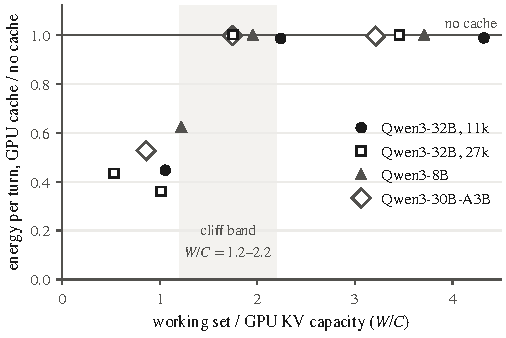
\includegraphics[width=\columnwidth]{../figures/wall.pdf}
\caption{GPU energy per turn with the GPU cache, relative to no cache, against the working set over the GPU's KV
capacity ($W/C$, with $W$ summing each session's largest prompt in the step), for three models and two context
lengths (vLLM, 5\,s pauses). Up to $W/C\approx1.2$ the cache saves 38--64\%; from 1.75 on the ratio is 1 within 2\%
in every case. Shaded: the band $\kappa=1.2$--2.2 in which hits collapse. At $W/C\approx1.75$ the 27k (16 sessions) and 30B-A3B (96 sessions) points coincide.}
\label{fig:wall}
\end{figure}

\paragraph{Eviction policy does not move the cliff.} Replacing LRU with LFU or SLRU left synthetic thrashing unchanged
(within 0.2\% of LRU in energy per turn at 48 and 96 sessions), consistent with the simulation of Lu et~al., in which even next-call-oracle eviction recovered only
1.08--1.18$\times$ LRU's goodput~\cite{lu2026metastability}, and with Liu et~al., who found on production traces from two
companies that 14 eviction algorithms gave little benefit over LRU~\cite{liu2026fancyevict}. On recorded trajectories at 48 sessions both cost 20--28\% more than
LRU.

\paragraph{Real trajectories are gentler.} Recorded SWE-agent sessions share one system prompt and start small. The GPU
cache kept 88\%, 85\% and 68\% of prompt tokens at 16, 48 and 96 sessions and still 72--73\% at 192 and 288, where we
had predicted under 30\%. Our synthetic sessions, with no shared prefix and steady growth, overstate collapse for these
2024 trajectories, whose final contexts are about 12k tokens. Production coding agents now carry far longer contexts
(a median of 68k prompt tokens per call in GitHub Copilot's traces~\cite{copilot2026wild}), which by Eq.~\eqref{eq:cliff} moves
them toward the long-context case above.

\section{Host-memory tiers}
\label{sec:tiers}

A host tier moves the cliff by enlarging the effective capacity, and Eq.~\eqref{eq:restore} says it should cost little
to use. Whether it helps depends on whether it holds the working set, as Shao et~al.\ showed for
run time~\cite{shao2026efficientagent}; we measure how much energy it saves as a function of its size
(Table~\ref{tab:tiers}).

\begin{table}[t]
\centering\small
\caption{SGLang host tiers, Qwen3-32B, synthetic sessions, 5\,s pauses (two rounds). WT: write-through; WB: write-back. $N$: sessions; Hit: hit rate. GPU cache alone:
0.12\% hit and 1,058\,J per turn at 48 sessions, 0.09\% and 1,035\,J at 96. vs.\ GPU: change in J/turn against the GPU cache alone at the same load. Where the two rounds differ at the precision shown, both values are given.}
\label{tab:tiers}
\begin{tabular}{lrrrr}
\toprule
Tier & $N$ & Hit & J/turn & vs.\ GPU \\
\midrule
80\,GB WT & 48 & 11.4--12.6\% & 953--962 & $-10$ to $-9\%$ \\
80\,GB WB & 48 & 36.5\% & 768 & $-27\%$ \\
120\,GB WT & 48 & 49.9--50.3\% & 652--655 & $-38\%$ \\
160\,GB WT & 48 & 75.5\% & 450 & $-57\%$ \\
240\,GB WT & 48 & 75.5\% & 448--449 & $-58\%$ \\
160\,GB WT & 96 & 20.2\% & 873 & $-16\%$ \\
240\,GB WT & 96 & 37.2\% & 732 & $-29\%$ \\
\bottomrule
\end{tabular}
\end{table}

\paragraph{Size against the working set.}\enlargethispage{\baselineskip} At 48 sessions the working set is about 548k tokens. SGLang's write-through
tier mirrors the GPU, so its usable capacity is roughly the host size rather than the sum of host and
GPU~\cite{lu2026metastability}: 80\,GB holds about 305k tokens ($W/C_{\text{host}}\approx1.8$, past the cliff) and saved 9--10\%; 160\,GB
holds about 610k ($W/C_{\text{host}}\approx0.9$) and saved 57\% with 84\% more turns and a median time to first token of 9\,s
instead of 55\,s. A 240\,GB tier added nothing at 48 sessions, because the set already fit, and saved 29\% at 96
sessions, where it did not. vLLM's host tier, which we could size only to 70\,GiB in our container, changed energy by $+0.3\%$ to $-6\%$.

\paragraph{A less inclusive tier gets more from the same memory.} In write-back mode SGLang copies KV to the host only
when it is evicted from the GPU, so the two tiers overlap less. At 80\,GB, write-back raised the hit rate from 11.4--12.6\%
to 36.5\% and cut energy per turn by 27\% instead of 9--10\%; at 160\,GB it matched write-through (not shown). On recorded
trajectories at 192 and 288 sessions an 80\,GB write-back tier came within 1.3--4.5\% of 160\,GB write-through
(68.8 against 67.9\,J and 62.1 against 59.4\,J per turn) with turn counts within 4.5\%: a less inclusive tier with half the host memory gave nearly the same
result.

\paragraph{Real trajectories.} On recorded SWE-agent sessions the 160\,GB tier lowered energy per turn by 33\% with
33\% more turns at 96 sessions against SGLang's GPU cache alone (91.5 against 136.6--138.2\,J), and by 27\% and 31\%
with 22\% and 27\% more turns at 192 and 288 sessions against vLLM's GPU cache (we did not run SGLang without a
tier at these loads). At 48 sessions, with no memory pressure yet, it
saved 3\%. These gains are smaller than on synthetic sessions because the GPU cache alone did not
collapse (Section~\ref{sec:cliff}).

\paragraph{How well the one-parameter model does.} With $f=0.76$ fitted on the 160\,GB, 48-session cell,
Eq.~\eqref{eq:energy} predicts the 80\,GB tier at 962\,J (measured 958, two-round means), vLLM's 70\,GiB tier at 1,035 and 973\,J (measured 1,035
and 973), and every other overloaded (48- and 96-session) synthetic Qwen3-32B host-tier cell within 1.4\% (2.5--3.4\% at 16
sessions), except one: 160\,GB at 48 sessions with 30\,s pauses, where it
predicts 534\,J and we measured 614\,J ($-13\%$). That cell drew 563\,W on average against 578\,W with 5\,s pauses: idle time likely dilutes
the prefill share, which the model, built for a busy card, does not capture; Section~\ref{sec:production} shows the same limit on production traffic at light load. On Qwen3-8B it predicts 207 and 254\,J for the 160\,GB tier at
128 and 256 sessions, against 215 and 266\,J measured ($-4$ to $-5\%$). On recorded trajectories,
where the GPU cache never thrashed, with no cache taken as $E_{\text{thrash}}$, it predicts the 160\,GB tier 6--23\% below the
measured energy per turn, so the fit does not transfer to those workloads.

\paragraph{Host cost.} We could not read the host's energy counters. From the engines' CPU time (charged at 10\,W per
busy core) and the bytes moved (assuming 1\,nJ per byte of host memory traffic) we estimate, under these assumed coefficients, the host's extra energy, as a
share of the GPU energy saved, at 0.5--1.8\% for the 160\,GB tier at 48 and 96 sessions and 2.9--3.0\% for 80\,GB at 48;
where the GPU saving was small the same estimate is larger: 11--14\% for SGLang tiers at 16 sessions and for 80\,GB at
96, 128\% for 80\,GB at 16 sessions with 30\,s pauses, and 4.7--212\% for vLLM's 70\,GiB tier. Mao and Zhou bounded the host-side cost at below 1\% of the GPU saving on a
similar host~\cite{mao2026offloading}.

\section{Production traffic}
\label{sec:production}

Synthetic sessions let us place the cliff; they do not say whether production traffic ever reaches it. The Kimi
tool-agent trace (Section~\ref{sec:setup}) answers that for one large deployment. Two of its properties matter. With
an unbounded cache, 55\% of its prompt blocks are reused, close to the 54--62\% Wang et~al.\ report for Alibaba's
traces~\cite{wang2025kvcachewild}. And requests in the same conversation return after a median of 114\,s (90th
percentile 420\,s): the gaps between a conversation's requests, which include tool
time, generation and queueing, last minutes, not the 5--30\,s pauses of our synthetic runs.

\paragraph{The host tier serves what the GPU cannot.} At a 1/4 sample (1,363 requests in the first window, 1,542 in the
second, about 11.5--12.2k prompt tokens per second) one H200 is past its capacity even with a cache
(Table~\ref{tab:prod}, Figure~\ref{fig:production}). With the GPU cache alone it finished 85--86\% of requests within the window plus 240\,s, with a
median TTFT of 89--200\,s; without a cache, 61--62\%. With a 160\,GB SGLang host tier it finished
every request in both windows, at 15--17\% less energy per prompt token than the GPU cache alone and about 40\% less than
no cache. The card averaged 585--590\,W under every policy, so total GPU energy over the window differed by at most
3.3\% between no cache, the GPU cache and the 160\,GB tier: the tier's gain is 16--18\% more prompt tokens finished for about the same energy, a gain in capacity. At the
1/8 sample, where every policy finished every request, the 160\,GB tier used 85.54\,mJ per prompt token against 86.08
for vLLM's GPU cache ($-0.6\%$; no SGLang GPU-cache run at 1/8). In the first window at 1/4, vLLM and SGLang with the GPU cache alone agreed to 0.1 points in hit rate and 1\% in energy, and the 160\,GB result
repeated within 0.1\% in a second round. A 300\,GB tier raised the hit rate by three more points, lowered energy by
another 4\% and cut the median TTFT from 129\,s to 107\,s.

\begin{table}[t]
\centering\small
\caption{Replay of Kimi's production tool-agent trace on one H200 (Qwen3-32B), 1/4 of the trace, 15-minute windows.
Done: requests finished within the window plus 240\,s. mJ/tok: all GPU energy of the window and drain divided by the prompt tokens of finished requests, which counts partial
work on unfinished requests and so raises the values of the policies that left requests unfinished. TTFT: median time to first token. Tiers are SGLang host tiers. Window: minutes of the trace replayed. Hit: prompt-token hit rate. Values are from one round; three first-window cells were repeated, and the repeats agreed within 0.2\% in energy and hit rate and 0.3\% in TTFT.}
\label{tab:prod}
\begin{tabular}{llrrrr}
\toprule
Window & Policy & Done & Hit & mJ/tok & TTFT \\
\midrule
0--15 & no cache (vLLM) & 61\% & 0\% & 104.4 & 270\,s \\
0--15 & GPU (vLLM) & 86\% & 36.7\% & 74.8 & 200\,s \\
0--15 & GPU (SGLang) & 86\% & 36.6\% & 75.6 & 199\,s \\
0--15 & 160\,GB (SGLang) & 100\% & 51.8\% & 62.8 & 129\,s \\
0--15 & 300\,GB (SGLang) & 100\% & 54.8\% & 60.3 & 107\,s \\
30--45 & no cache (vLLM) & 62\% & 0\% & 101.6 & 236\,s \\
30--45 & GPU (vLLM) & 85\% & 38.2\% & 71.9 & 89\,s \\
30--45 & 160\,GB (SGLang) & 100\% & 52.2\% & 61.3 & 67\,s \\
\bottomrule
\end{tabular}
\end{table}

\begin{figure}[t]
\centering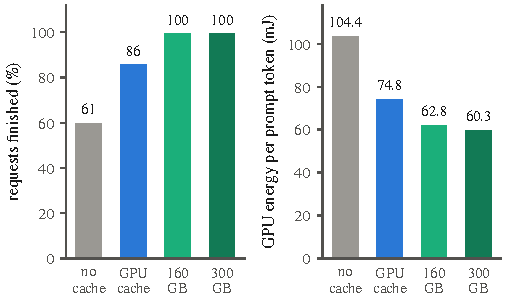
\includegraphics[width=\columnwidth]{../figures/production.pdf}
\caption{Kimi tool-agent trace, 1/4 sample, first window, one H200. Left: share of requests finished; right: GPU energy per
prompt token, which includes energy spent on unfinished requests (round 1, the values of Table~\ref{tab:prod}). No cache and GPU cache on vLLM; host tiers on SGLang.}
\label{fig:production}
\end{figure}

\paragraph{The energy model on production traffic.} Equation~\eqref{eq:energy}, with the $f=0.76$ fitted on synthetic
sessions, predicts the ratio of each policy's energy per prompt token to that of no cache from its measured hit rate.
On the busy card it is right to within about 1\%: 0.721 predicted against 0.717--0.718 measured for vLLM's GPU cache, 0.606
against 0.601 for 160\,GB and 0.584 against 0.578 for 300\,GB in the first window, and 0.709 against 0.708 for the GPU cache and 0.603 against 0.603 for 160\,GB
in the second. At a 1/8 sample, where the GPU cache ran well below full power (544\,W), the model fails: the GPU cache measured 0.847 of no-cache
energy where the model gives 0.653. There the window includes idle and decode-bound time, the prefill share is smaller
(the measured ratio implies $f\approx0.33$), and the cache's benefit is mostly latency: a median time to first token of
1.2\,s instead of 18\,s, and a 90th percentile of 7.1\,s instead of 77\,s.

\paragraph{Predicting the hit rate from logs.} Because the trace carries block hashes, the hit rate of any cache size
can be estimated offline by replaying the hashes through an LRU of that many blocks, as KVSET does with the Mattson
stack algorithm~\cite{kvset2026,mattson1970evaluation}. We wrote these predictions before each run. When the card kept
up (finished every request), they came within 0.6 points at 1/8 and 2.3--4.3 points at 1/4: 45.65\% measured against 46.25\% predicted for the GPU cache at 1/8 in the second window, 52.62\%
against 52.66\% for 160\,GB at 1/8, and 51.8\% and 54.8\% against 47.5\% and 52.5\% for 160 and 300\,GB at 1/4 in the first. When
the card was overloaded the predictor read high: 36.7\% measured against 41.8\% predicted, and 38.2\% against 44.7\%,
for the GPU cache alone at 1/4. A likely cause, which we did not measure, is that unfinished requests and queueing change which requests the cache
sees and in what order; a prediction from logs must therefore come with a capacity check.

From hashed request logs alone, which contain no prompt text, one can estimate what hit rate a given GPU and host
memory will reach when the card keeps up and, on a busy card, what that hit rate will save in energy. Chained, the
logged hit-rate prediction and Eq.~\eqref{eq:energy} put the two host tiers at 1/4 in the first window within 4--6\% of their measured
energy ratios.

\section{Admission control}
\label{sec:control}

If the working set will not fit, the server can still choose which sessions hold the memory. Equation~\eqref{eq:gate}
gives the size of the admitted set. We tested four versions of the gate and one published alternative, in the order we
built them; each failure led to the next version. We call them the static gate, the formula, the shared-prefix
formula and the adaptive gate.

\paragraph{A static gate saves energy and starves sessions.} Admitting 16 of 48 synthetic sessions, each for 4 or 8
turns, cut energy per turn by 41--47\% with 5\,s pauses. With 30\,s pauses, where a held slot sits idle for longer, it cost 6--8\% more at 48 sessions and 11--16\%
more at 96. Within a 150\,s step, 6--32 of 48 and 53--80 of 96 sessions were never served. Over 10 minutes, which lets the gate
rotate, the energy gain held, but the latency tail doubled: against the GPU cache alone (333 turns,
1,185\,J per turn, median resume latency 54\,s, 90th percentile 70\,s), the gate gave 456 turns at 761\,J with a median of 1.4\,s
and a 90th percentile of about 146\,s.

\paragraph{The formula and an AIMD window.} Setting $K$ from the engine's reported capacity and the recent size
of sessions, recomputed every 2\,s, saved 40\% and 31\% at 48 and 96 sessions with 5\,s pauses, and 7\% and 1\% with 30\,s pauses. In 150\,s steps it
served only 20 of 48 and 21 of 96 sessions, so part of the gain may have come from serving fewer of them; over 10 minutes at 48
sessions it gave 500 turns at 682\,J, with a median resume latency of 0.5\,s and a 90th percentile of about 147\,s. A CONCUR-style AIMD
window~\cite{chen2026concur}, in our reimplementation with CONCUR's published parameters, saved at most 1.3\% in this
closed-loop setting on synthetic sessions (on recorded trajectories it saved 5\% at 96 sessions and cost 6\% more at
48). On synthetic sessions its window rose to 44 in the first minute, then fell by repeated halving to 1 and stayed
near 1 for the rest of most steps; on recorded trajectories it only grew, to 158, never halving, as did the CONCUR-inspired controller that He
reports~\cite{he2026robot}. This does not test CONCUR itself, whose evaluation is offline batch inference.

\paragraph{Real agents broke the first formula.} Sized from the 90th percentile of recent prompts, the formula admitted
too few recorded SWE-agent sessions: they share a system prompt, which the engine stores once, so the per-session cost
is far below the prompt length. At 192 and 288 sessions it raised energy per turn by 31\% against the GPU cache alone
and served 40--50\% fewer turns. The shared-prefix formula, which subtracts the shared prefix and sizes from the mean (Eq.~\eqref{eq:gate}), reversed
this: $-13\%$ and $-15\%$ against the GPU cache (80.2 and 73.0 against 92.4 and 85.6\,J per turn), with hits 8.5--9.6
points higher and 1.5\% and 8\% fewer turns, repeated within 1.5\% in a second round. On the MoE model, whose GPU cache
never collapsed on these trajectories, the shared-prefix formula changed energy by $+0.3\%$ to $-2.5\%$ and cut the 90th
percentile of resume latency at 192 sessions from 0.37 to 0.22\,s.

\paragraph{A gate next to a host tier.} Combined with a 160\,GB host tier, which on
real trajectories already held 89--91\% of tokens, the shared-prefix formula cost 10\% more energy at 192 sessions and nothing at 288,
against the tier alone, and served 15--18\% fewer turns. We had predicted a further 25\% saving. This run is flawed: its
gate was sized to the GPU's 251k-token capacity instead of the tier's 610k (the trajectory driver preferred the engine's reported capacity to the configured one; the run records the GPU
value), so it
admitted a median of about 100 sessions at a time (24--280 over a step) of the 192--288 open; it shows only that a gate sized to the GPU should not front a host tier. On synthetic sessions, where the tier alone reached only
35\% hits at 96 sessions over 10 minutes, the original (90th-percentile) formula with a 160\,GB tier, sized to the tier, cut energy per turn by 36\% with 34.5\% more turns,
served all 96 sessions and moved the median resume latency from 110\,s to 16\,s at the price of a longer tail (204\,s
against 124\,s at the 90th percentile). A gate helps only when memory is short.

\paragraph{An adaptive gate.} The last version applies $K$ only when the open sessions' working set exceeds
$\theta C$ with $\theta=1.2$, and otherwise admits everyone. We registered its predictions before running it on two
workloads, two rounds each (Table~\ref{tab:adaptive}, Figure~\ref{fig:adaptive}). Below the cliff it matched the GPU cache in energy (within
0.2\% at 4 and 8 long-context sessions) and in latency (on Qwen3-8B at 64 sessions the switch turned the gate on in
about a fifth of its 2\,s control intervals, so a few resumed turns waited up to 17\,s for readmission); the formula alone had cost up to 2.7\% more energy at long context and, on
Qwen3-8B at 64 sessions, used 9\% less energy than the GPU cache but had a 90th-percentile resume latency of 8--12\,s instead of 1.6--1.9\,s. Above the cliff it took the full
gain of the formula: 41\% less energy per turn on Qwen3-8B at 128 and 256 sessions and 44--45\% at 16 and 32
long-context sessions, with 90th-percentile resume latency falling from 24--81\,s to 0.6--1.5\,s and from 40--121\,s to
8.7--12.7\,s. Every registered threshold held. At 4 and 8 long-context sessions the switch never turned the gate on, so
those cells ran as the GPU cache; the switch changed state only on Qwen3-8B at 64 sessions. We did not test $\theta=1.2$ with
30\,s pauses, where hits persist to $W/C\approx1.86$, nor on recorded or production traffic.

\begin{figure*}[t]
\centering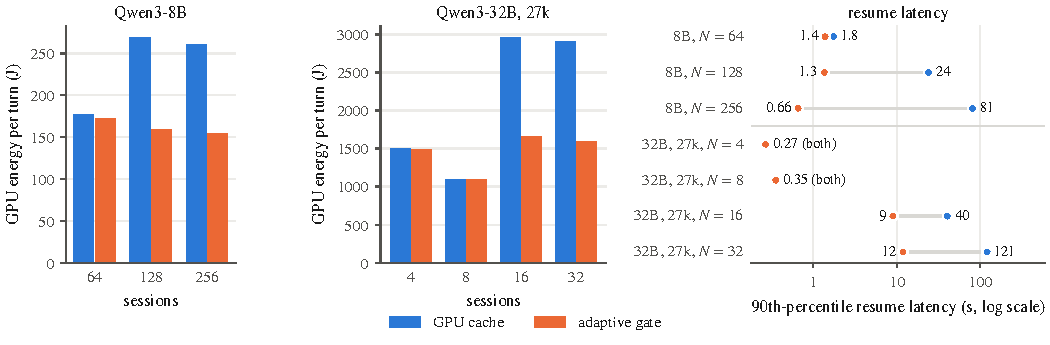
\includegraphics[width=\textwidth]{../figures/adaptive.pdf}
\caption{The adaptive gate against the GPU cache alone, for both workloads of Table~\ref{tab:adaptive} (vLLM, 5\,s
pauses, 150\,s steps). Left and middle: measured GPU energy per turn, mean of two rounds (the two rounds agree within 1.5\% in
every cell). Right: 90th percentile of resume latency, one row per cell (mean of two rounds; turns after a session's
first), including any wait for admission, on a log scale. Below the cliff (8B at 64 sessions, 32B at 4 and 8) the two policies are within 3\% in energy; above
it the gate cuts energy by 41--45\% and the tail of resume latency by 4.5--123$\times$;
first admissions wait longer and fewer sessions are served at the highest loads (Section~\ref{sec:control}).}
\label{fig:adaptive}
\end{figure*}

These latency figures, like the registered thresholds, cover resumed turns; admission waits fall mostly on first
turns. Above the cliff the 90th percentile of first-turn latency was 88--91\,s and 130\,s with the gate on Qwen3-8B at
128 and 256 sessions (38 and 88\,s with the GPU cache alone) and 112--113 and 110--114\,s at 16 and 32 long-context sessions (62
and 132\,s): longer in three of the four cells over the sessions served, and in all four once the sessions never served,
each waiting at least 143\,s, are counted. At the two highest loads the gate served only 170 of 256 and 16--17 of 32 sessions within the 150\,s step,
where the GPU cache served all of them, so part of its energy gain there may come from serving fewer sessions, as with
the static gate (in 600\,s steps, with every session served, the gain held). Over all turns of the sessions served, its 90th-percentile latency was 68--86\,s against 30--82\,s
for the GPU cache on Qwen3-8B and 77--82\,s against 54--122\,s at long context. 
\paragraph{Ten-minute steps.} To see whether rotation closes this gap, we registered a further prediction (H28)
and ran the gate and the GPU cache for 600\,s at the two loads where sessions went unserved, one round, on a second
H200 NVL host with the same engine and meter versions (Table~\ref{tab:tenmin}); a third registered cell, Qwen3-8B at 128 sessions, was
dropped for budget reasons before any data were collected. The 10-minute baselines, on the second host, used more energy per turn than the 150\,s baselines on the first (292 against
261\,J on Qwen3-8B, 3,022 against 2,901\,J at long context). With rotation the gate served every session,
completed 48\% and 62\% more turns and cut energy per turn by 42\% and 50\%; no session completed fewer turns than
under the GPU cache. The cost is queueing: the 90th percentile of first-turn latency was 183 against 68\,s and 253
against 131\,s, and of resumed turns including readmission waits 226 against 102\,s and 251 against 130\,s. H28's
energy and served-sessions clauses held; its latency clause (at most 1.5 times the GPU cache's first-turn tail) did
not. In these two 10-minute runs the gate traded first-turn latency, rather than sessions served, for throughput and energy.


\begin{table}[t]
\centering\small
\caption{The adaptive gate against the GPU cache alone (vLLM, 5\,s pauses, 150\,s steps, two rounds). $N$: sessions. J/turn: energy per turn, mean of the two rounds. p90: 90th
percentile of resume latency (turns after a session's first) including any wait for admission, as a range over the two rounds, or one value where they agree at the precision shown.}
\label{tab:adaptive}
\setlength{\tabcolsep}{3pt}
\begin{tabular}{lrrrrr}
\toprule
Workload & $N$ & \multicolumn{2}{c}{J/turn} & \multicolumn{2}{c}{p90} \\
\cmidrule(lr){3-4}\cmidrule(lr){5-6}
 & & GPU & adaptive & GPU & adaptive \\
\midrule
Qwen3-8B & 64 & 176.6 & 171.9 & 1.6--1.9\,s & 1.3--1.5\,s \\
Qwen3-8B & 128 & 269.6 & 159.6 & 24\,s & 1.2--1.5\,s \\
Qwen3-8B & 256 & 261.3 & 154.5 & 81\,s & 0.6--0.7\,s \\
Qwen3-32B, 27k & 4 & 1,495 & 1,494 & 0.27--0.28\,s & 0.26--0.28\,s \\
Qwen3-32B, 27k & 8 & 1,095 & 1,094 & 0.35--0.36\,s & 0.35--0.36\,s \\
Qwen3-32B, 27k & 16 & 2,964 & 1,658 & 40\,s & 8.7--9.2\,s \\
Qwen3-32B, 27k & 32 & 2,901 & 1,589 & 121\,s & 11.0--12.7\,s \\
\bottomrule
\end{tabular}
\end{table}

\begin{table}[t]
\centering\small
\caption{The adaptive gate in 600\,s steps (vLLM, 5\,s pauses, one round, second host). $N$: sessions. Served: sessions with at
least one turn. Min.\ turns: fewest turns any session completed. p90 first: 90th percentile of first-turn latency including
admission waits. Gate: the adaptive gate.}
\label{tab:tenmin}
\setlength{\tabcolsep}{2.4pt}
\begin{tabular}{lrlrrrrr}
\toprule
Workload & $N$ & Policy & Served & Turns & J/turn & Min. & p90 \\
 & & & & & & turns & first \\
\midrule
Qwen3-8B & 256 & GPU & 256 & 1,436 & 292 & 5 & 68\,s \\
 & & gate & 256 & 2,119 & 168 & 6 & 183\,s \\
Qwen3-32B, 27k & 32 & GPU & 32 & 143 & 3,022 & 4 & 131\,s \\
 & & gate & 32 & 232 & 1,507 & 4 & 253\,s \\
\bottomrule
\end{tabular}
\end{table}

The adaptive gate is a working-set admission rule with a switch; it is not a new idea in kind (Section~\ref{sec:related}).
The measurements show where each part helps: the shared-prefix term on real agents, the switch below the cliff, where it keeps latency at the GPU cache's level, and
the formula above it, with its gain in joules and its cost at admission. A correctly sized gate next to a host tier
that already holds the working set remains untested on real trajectories.

\section{Correct answers per kilowatt-hour}
\label{sec:accuracy}

Energy per token says nothing about whether an agent still gets its tasks right. Caching should not change
outputs in principle, but we did not assume runs with and without it are identical, so we measured accuracy directly on 400 graded multi-turn tasks of BFCL~v4~\cite{bfcl2025} (base and long-context), with the benchmark's own grader and Qwen3-32B on vLLM, and recorded the GPU energy of each whole run
(Table~\ref{tab:bfcl}).

\begin{table}[t]
\centering\small
\caption{BFCL v4 multi-turn, Qwen3-32B on vLLM, 400 tasks (200 base, 200 long-context), 100 at a time, one round. Correct: total (base\,/\,long-context). Per kWh: correct tasks per kWh of GPU energy.}
\label{tab:bfcl}
\begin{tabular}{lrrrr}
\toprule
 & Correct & Time & Energy & Per kWh \\
 & & (min) & (kWh) & \\
\midrule
GPU cache & 204 (113\,/\,91) & 64 & 0.619 & 330 \\
no cache & 201 (120\,/\,81) & 129 & 1.239 & 162 \\
\bottomrule
\end{tabular}
\end{table}

Accuracy differed by 3 of 400 tasks (204 against 201), with category-level differences of 7--10 tasks in opposite
directions; with one round we cannot separate a cache effect from run-to-run variation. With the cache the same graded work took half
the time and half the GPU energy, so it produced 2.0$\times$ the correct answers per kWh. We had predicted equal accuracy
within two points and at least 20\% less energy per correct task; the energy per correct task fell by 51\%. A second
round was dropped for budget reasons. In both runs 23--24 long-context tasks were rejected by the engine because the
conversation exceeded the 40,960-token context (HTTP 400) and were counted as incorrect, which lowers absolute accuracy for both policies alike.

\section{Related work}
\label{sec:related}

\paragraph{KV caching and memory tiers.} PagedAttention~\cite{kwon2023pagedattention} manages KV memory in pages and
lets vLLM share blocks across requests; SGLang's RadixAttention~\cite{zheng2024sglang} keeps finished requests' KV in a
radix tree under LRU\@. Pensieve~\cite{yu2025pensieve} and CachedAttention~\cite{gao2024cachedattention} keep
multi-turn state across a GPU and a host tier, and Mooncake~\cite{qin2024mooncake}, LMCache~\cite{liu2025lmcache} and
SGLang's HiCache~\cite{xie2025hicache} provide host or disaggregated tiers in production engines. Meng
et~al.~\cite{meng2025bottlenecks} show that offloaded serving can be bound by PCIe. These systems report latency,
throughput or cost. Lu et~al.\ already treat a write-through HiCache tier as inclusive, with capacity
$\max(C, C_{\text{host}})$~\cite{lu2026metastability}.

\paragraph{Agents, thrashing and tiers.} InferCept~\cite{abhyankar2024infercept} chooses among discarding, preserving
and swapping context during tool calls; Continuum~\cite{li2025continuum} pins KV with a time-to-live; CacheWise~\cite{tiwari2026cachewise}
uses reuse-aware eviction for coding agents; MARS~\cite{wang2026mars} keeps KV only when a warm resume shortens the
critical path. TokenCake~\cite{tokencake2025} moves idle KV to host memory when a function call starts, if the freed memory can be used, and
MORI~\cite{xia2026mori} ranks agent programs by idleness and places the most idle in host memory, reporting 20--71\%
higher throughput on Claude Code traces. CONCUR~\cite{chen2026concur} names middle-phase thrashing and controls it with
an AIMD window; He~\cite{he2026robot} reports a sharp retention boundary under cyclic revisits (between 28 and 32 sessions of 100k tokens in a 3.35M-token pool,
just below $C/s$) and avoids the thrashing with a static cap; Lu et~al.~\cite{lu2026metastability} fit the cliff at $1.9\,C/\bar c$, with $\bar c$ the mean context, in a disaggregated engine and admit
sessions against a working-set budget (Basin); concurrently, Valse and Jannesari~\cite{valse2026trap} show that a burst can
trap an engine in a state where every turn misses, model that state with a renewal law and rescue it with a session
cap, reporting hits and throughput rather than energy; Shao et~al.~\cite{shao2026efficientagent} show that a host tier pays
off only when it holds the reuse working set, sized with a stack-distance model. TAO~\cite{li2026tao} jointly selects
and places waiting sessions. Our admission gate is a working-set rule in the same
family; we add the energy measurements and the shared-prefix correction (Basin already switches its admission on only
above a working-set threshold), and we report where each version failed.

\paragraph{Traces and hit-rate prediction.} Wang et~al.\ characterize two weeks of Alibaba's KV reuse and find ideal
hit rates of 54--62\%~\cite{wang2025kvcachewild}. Agentic coding traces from GitHub Copilot~\cite{copilot2026wild} and
TraceLab~\cite{tracelab2026} show long contexts and long idle gaps, and Khailo~\cite{keepalive2026} prices
keeping prefixes warm across pauses. KVSET~\cite{kvset2026} estimates hit rate against capacity from traces with the
Mattson stack algorithm~\cite{mattson1970evaluation} and validates it with a production coding-agent trace against cache pools of several sizes;
Yao et~al.~\cite{yao2026lrumeanfield} derive a closed-form limit of the LRU hit ratio for multi-turn conversations and an
estimator for memory provisioning. Our block-LRU
predictor is the same idea; what we add is its check against a GPU in both regimes (it holds when the card keeps up and
reads high under overload) and the energy model on top of it.

\paragraph{Energy of serving.} Serving energy is benchmarked routinely~\cite{chung2025mlenergy,pronk2025benchmarking,
zine2026attention,luo2026request}, and the carbon cost of caching and of agents has been modelled and optimized~\cite{greencache2025,agentdecarbonizer2026}.
PrefixBench-H100~\cite{shewale2026prefixbench} reports 24--31\% less energy per request from prefix reuse (20--24\% in its own table) at
concurrency 1; Librarian~\cite{cho2026librarian} fits 34\,mJ per uncached and 2\,mJ per cached input token for a 27B model
in FP8 on a B200; the SIMPLE law~\cite{cavagna2026simple} estimates that prefix caching removes 93\% of agentic prefill
energy. Luo et~al.~\cite{luo2026where} show that, on their agent server, GPU-only telemetry missed 41--45\% of the energy. Closest
to us, Mao and Zhou~\cite{mao2026offloading} measure vLLM's KV offloading on an H200 at concurrency 2--6 and find 14--32\%
savings only above about 90\% KV utilization, with a host-side cost bounded below 1\% of the GPU saving; they estimate restore
to be at least 400$\times$ cheaper per byte than recompute. The llm-d agenda~\cite{sisodia2026toward} asks when
transfer is greener than recompute. We answer it for one case, restoring from host memory over PCIe, by measurement, through the collapse and on production
traffic.

\paragraph{Classic results.} Our explanations are textbook ones: Belady's optimal replacement~\cite{belady1966study},
Denning's working set and thrashing~\cite{denning1968working,denning1968thrashing}, LRU's failure on cyclic patterns
and its fixes~\cite{jiang2002lirs,megiddo2003arc}, and Wong and Wilkes on inclusive versus exclusive two-level
caches~\cite{wong2002mycache}, whose analysis predicts our write-back result. Prior serving work already draws these parallels;
we claim no novelty for them.

\section{Discussion}
\label{sec:discussion}

\paragraph{Longer contexts lower the cliff.} Equation~\eqref{eq:cliff} with $\kappa$ between 1.2 and 2.2 gives a rough count
of the agents a card can hold before its cache stops paying. For a 32B model in BF16 and sessions of 68k tokens, the
median reported for GitHub Copilot's agent traces~\cite{copilot2026wild}, it gives about 4--8 sessions on an H200, 7--13 on a
192\,GB card and 13--24 on a 288\,GB card. These are projections, not measurements: our measurements support the
model at about 11k and 27k tokens on one card. If agent contexts keep growing faster than HBM capacity, the number of agents a card can hold will fall, and host tiers and
admission control will matter more.

\paragraph{Energy, capacity and money.} For an operator who rents GPUs, the energy saved is worth little in itself:
at its 600\,W maximum board power~\cite{nvidia2024h200} an H200 NVL draws about 440\,kWh a month, about \$44 at an assumed \$0.10 per kWh, while the card we rented
cost \$3.71 an hour, about \$2,700 a month. What the results buy is capacity. Finishing every production request
instead of 85--86\%, or serving 22--33\% more recorded agent turns, amounts to needing fewer GPUs. Where power, not
GPUs, limits a deployment, lower energy per turn means more turns from the same power.

\paragraph{Limitations.}
\label{sec:limits}
All results come from one GPU type (H200 NVL) in one rented container (the 10-minute adaptive-gate runs in a second container), with one model family. Energy is GPU board
energy only: host CPU and memory were not metered, and system-level savings can be proportionally smaller, since on one agent server GPU telemetry
missed 41--45\% of the energy~\cite{luo2026where}. The pauses of the recorded trajectories are synthetic, because the dataset has
no tool timings; the production trace has real timing but synthetic token contents, which preserve sharing and length
but not, for example, any effect of content on decoding. One GPU cannot carry the production trace, so we replayed
1/8 and 1/4 samples by prefix group. The admission results use
synthetic sessions or recorded trajectories, not a live agent framework, and the adaptive gate needs to know how many
sessions are open; its switch was tested only with 5\,s pauses. The miss-penalty sweep, BFCL, most production cells, the long-context no-cache baseline, the 10-minute adaptive-gate runs and SGLang's GPU cache
with Qwen3-8B ran one round. In the production replay, energy per prompt token counts all energy but only finished
requests' tokens, which favors policies that finish more requests; the 15--17\% host-tier gain includes this effect,
which we did not separate. One block of runs was
discarded after two copies of a run script shared the GPU; no result in this paper comes from it.

\section{Conclusion}

Below the cliff the GPU cache saved 38--64\% of GPU energy per turn on synthetic sessions with 5\,s pauses; past it, energy per turn was within
0.01--1.6\% of running without a cache, because a thrashing cache does the same work as no cache. The cliff follows from capacity and session size, with a measured factor of 1.2--2.2 that was larger with 30\,s than with 5\,s pauses, and
moves inward as contexts grow. A 1/4 sample of production tool-agent traffic pushed one GPU past its capacity, and a 160\,GB host tier
let it finish every request: 16--18\% more prompt tokens for about the same GPU board energy. Restoring KV took
1/110 to 1/220 of the above-idle GPU energy of recomputing it, holding it cost no measurable power, and a gate that
acts only under pressure cost no energy below the cliff and, in two 10-minute runs above it, served every session with
42--50\% less energy per turn and 48--62\% more turns, at the price of minutes of queueing at admission. On a busy GPU that keeps up, the energy effect of a host tier
can be estimated from hashed request logs before a server is changed: within 4--6\% for the two tiers we tested on production traffic.


\bibliographystyle{plainnat}
\bibliography{../references}

\appendix
\onecolumn
\section{Pre-registered hypotheses and verdicts}
\label{app:prereg}

Each hypothesis in Table~\ref{tab:prereg} was written into a plan document, most with a numeric threshold (H4 and H8 had none), before the runs that tested it.
The plan is under version control; the time given is that of the commit that added the prediction, which precedes the
first run that tested it. Several predictions were added during the study, after earlier runs, and the plan says which
results had been seen when each was written. Verdicts were added in later commits; no prediction was edited after its first run.
``Not supported'' means the registered threshold was missed, even when the direction was right; ``Partly'' means
some clauses or cells held and others did not. The shared-prefix formula (7~Nov 02:43) was written after H16
and H21 and was the formula their runs used.
\begin{table}[p]
\centering\footnotesize
\renewcommand{\arraystretch}{1.0}
\caption{Pre-registered hypotheses (abridged), commit time (UTC, 2026) and outcome. Rows follow the plan's numbering;
where two times are given, a clause was added or reworded, or a cell dropped, in a later commit, before the runs that tested it.}
\label{tab:prereg}
\begin{tabular}{p{0.03\textwidth}>{\raggedright\arraybackslash}p{0.125\textwidth}>{\raggedright\arraybackslash}p{0.36\textwidth}>{\raggedright\arraybackslash}p{0.41\textwidth}}
\toprule
& Written & Prediction & Outcome \\
\midrule
H1 & 5 Nov 15:36 & vLLM and SGLang within 3\% in energy per output token, default and tuned & Partly: defaults within 2.3\%; tuned settings differ by up to 5.7\% on a retrieval-style workload (one SGLang scheduling flag), in an open-loop chat and retrieval comparison run before the agent study and not otherwise reported \\
H2 & 5 Nov 15:36 & Miss/hit energy penalty $\le$1.5$\times$ at 1 user, $\ge$5$\times$ at 64 users & Supported: 1.46--1.48$\times$ and 10.1--10.6$\times$, both engines \\
H3 & 5 Nov 15:36, 23:29 & An 80\,GB host tier cuts energy per turn $\ge$20\% at 48 sessions & Not supported: $-10$ to $-9\%$ (inclusive tier smaller than the working set) \\
H4 & 5 Nov 15:36 & Longer pauses make offload more useful & Not supported as stated (no threshold): unchanged, smaller or larger by engine and size \\
H5 & 5 Nov 15:36 & Host-side cost of offloading $<$10\% of the GPU saving & Partly (an estimate): 0.5--3\% where SGLang tiers saved most; 11--128\% for SGLang tiers and 4.7--212\% for vLLM 70\,GiB where savings were small \\
H6 & 6 Nov 02:07 & A gate of 16 slots: hit $\ge$30\%, energy $\ge$25\% lower at 48 sessions, both pause lengths & Partly: supported at 5\,s ($-41$ to $-47\%$); not at 30\,s ($+6$ to $+8\%$ at 48) \\
H7 & 6 Nov 02:14 & LFU keeps $\ge$20\% hit at 48 sessions; SLRU collapses ($<$5\%) & Partly: LFU not supported (0.21\%); SLRU supported; both within 0.2\% of LRU in energy; 20--28\% worse on real trajectories \\
H8 & 6 Nov 02:48 & Fit hit rate against $W/C$ to the fixed-cycle ($\kappa=1$) and random-order ($\kappa\approx1.58$) models (no threshold) & No threshold: neither fits both; resumed-turn hits halve (from their 16-session level) at $W/C\approx1.2$ (5\,s) and 1.5 (30\,s), vanish by 1.55 and 2.2 \\
H9 & 6 Nov 02:56 & A 160\,GB tier: hit $\ge$50\%, energy $\ge$20\% lower at 48 sessions; $<$10\% saving at 96 & Partly: $-57\%$ at 48; $-16\%$ at 96 (threshold missed) \\
H10 & 6 Nov 03:23 & Restore $\le$1/10 of recompute per token & Supported: 1/110 to 1/220 \\
H11 & 6 Nov 09:30 & Holding a full cache costs $<$2\% idle power & Supported: $-0.08$ to $-0.16\%$ \\
H12 & 6 Nov 12:59 & BFCL: accuracy within 2 points; $\ge$20\% less energy per correct task & Supported (one round): 204 vs.\ 201, $-51\%$ \\
H13 & 6 Nov 05:09 & Formula saves $\ge$30\% and beats AIMD & Partly: $-40\%$, $-31\%$ at 48, 96 sessions (5\,s pauses), $-7\%$, $-1\%$ (30\,s); below AIMD in 3 of 4 cells; AIMD 0.55\% lower in the fourth \\
H14 & 6 Nov 05:34, 18:02 & Real trajectories collapse at 96 (later: 192--288) sessions; formula (at 96) and 160\,GB tier (at 48) each $\ge$20\% (later: both at 192--288) & Partly: no collapse (68\% hit at 96, 72--73\% at 192--288); formula $-12$ to $-13\%$ at 96, $+31\%$ at 192--288; 160\,GB tier $-3\%$ at 48 (missed), $-27\%$, $-31\%$ at 192, 288 \\
H15 & 6 Nov 06:20 & No time-based eviction & Supported: resends after 25\,min fully cached \\
H16 & 6 Nov 09:30 & MoE: same cliff; formula $\ge$20\% on real agents & Partly: cliff and thrash = no cache held; formula clause not (no collapse) \\
H17 & 6 Nov 13:35, 23:58 & 120\,GB: 10--40\% hit; 240\,GB: $\ge$75\% hit at 48, 15--50\% hit and $\ge$35\% saving at 96; 160\,GB tier with the formula $\ge$60\% hit & Partly: 120\,GB 50\% and 240\,GB at 96 $-29\%$ missed; 240\,GB hits 75.5\%, 37.2\% and tier with formula 75\% held (49 of 96 sessions served) \\
H18 & 6 Nov 13:40 & Write-back beats write-through at 80\,GB (at 50\% hit, about half the RAM for the same benefit); within 10\% at 160\,GB & Partly: 11.4--12.6\% $\to$ 36.5\%, $-27\%$ energy; 50\% mark not reached; 160\,GB equal \\
H19 & 7 Nov 01:29 & 160\,GB + gate, 10-min steps: all served, $\ge$30\% below 160\,GB alone & Supported: 96/96 served, $-36\%$, $+34.5\%$ turns \\
H20 & 7 Nov 01:29 & 80\,GB write-back + gate within 15\% of 160\,GB + gate & Not supported: $+20$ to $+21\%$ (gate capacity set to 420k tokens) \\
H21 & 7 Nov 01:29 & 160\,GB + gate $\ge$25\% below 160\,GB alone on real agents; 80\,GB WB between GPU cache and 160\,GB & Partly: $+10\%$ and 0\% (gate sized to the GPU, not the tier; Section~\ref{sec:control}); write-back clause supported \\
H22 & 7 Nov 01:29 & Qwen3-8B: cliff near $C/s$ (hit $>$60\% at 64, $<$5\% at 256); tier and formula each $\ge$30\% & Partly: cliff thresholds and formula ($-41\%$) supported; tier not ($-20\%$, $+2\%$) \\
H23 & 7 Nov 04:27 & Production hit within 5 points of block-LRU prediction & Partly: 2 of 3 cells (window 1); 0.04--0.6 points at 1/8 (window 2); overload misses \\
H24 & 7 Nov 04:27 & No cache cannot keep up; GPU cache finishes $\ge$98\% & Partly: no cache 61--62\%; GPU cache only 85--86\% \\
H25 & 7 Nov 04:27 & GPU cache $\le$0.70$\times$ no-cache energy per token; tiers follow Eq.~\eqref{eq:energy} within 5\% & Partly: 0.717--0.718 (missed); tiers within 1\% \\
H26 & 7 Nov 18:51 & Long context: hit $\ge$85\% at 4, $\ge$70\% at 8, $<$5\% at 32 with energy within 3\% of no cache & Supported \\
H27 & 7 Nov 18:51 & Adaptive gate: no cost below the cliff, formula's gain above & Supported: every cell, both workloads, both rounds (resumed turns) \\
H28 & 8 Nov 18:55, 19:15 & Adaptive gate, 600\,s steps: $\ge$75\% served, $\ge$30\% less energy, first-turn p90 $\le$1.5$\times$ GPU cache & Partly: 100\% served, $-42\%$ and $-50\%$; first-turn p90 2.7$\times$ and 1.9$\times$ \\
\bottomrule
\end{tabular}
\end{table}




\section{Derivation details}
\label{app:derive}

\paragraph{FLOP per token.} Qwen3-32B has hidden size 5,120, 64 layers, 64 query and 8 KV heads of dimension 128, and an
MLP of width 25,600; its 31.2 billion non-embedding parameters give 62.4\,GFLOP per token. Attention scores and the
weighted sum of values each cost $2\times64\times128$ FLOP per layer per earlier token, together 2.10\,MFLOP over 64 layers.

\paragraph{Random-order cliff.} As a mean-field approximation, let a session be away for exactly one mean cycle while
each of the other $N-1$ sessions returns as a Poisson process with that mean interval. Each is then touched during the
absence with probability $1-1/e\approx0.63$, and the session survives if $s(1 + 0.63(N-1)) \le C$, which gives
$N^\ast \approx 1 + (C/s-1)/0.63$: a factor that approaches $1/(1-1/e)\approx1.58$ over the cyclic case $N^\ast=C/s$ as
$C/s$ grows (1.56 at $C/s=23$). With exponential absences the expected share touched falls to $1/2$
and the hit rate declines gradually; our measured drops are sharper than that.

\paragraph{Projection for long contexts.} For Qwen3-32B in BF16 ($b_{\text{KV}}=262{,}144$\,bytes, 65.5\,GB of weights,
$u=0.9$), Eq.~\eqref{eq:cliff} gives $C\approx234$k tokens at 141\,GB (the engine reported 245k), 409k at 192\,GB and
739k at 288\,GB; with $s=68$k tokens and $\kappa=1.2$--2.2, it gives 4--8, 7--13 and 13--24 sessions.


\end{document}
